\chapter{Agent Based Modelling}

Multi-agent systems are applied in various domains to replicate commplex systems with:
\begin{itemize}
    \item Multiple artificial or natural entities;
    \item Interactions among entities that produce emergent behaviors;
    \item The \textbf{microscopic} model is not sufficient to predict global system behavior;
    \item The focus is on \textbf{macroscopic} behavior.
\end{itemize}

\begin{definitionblock}[Agent-Based Modelling (ABM)]
    Agent-Based Modelling (ABM) is a computational approach for simulating the interactions of autonomous agents to assess their effects on the system as a whole.
\end{definitionblock}

It is:
\begin{itemize}
    \item \textbf{Versatile and Heterogeneous}, since agents can represent different entities with diverse behaviors and attributes;
    \item \textbf{Agnostic}, since any architecture can be used and programmed in any language;
    \item \textbf{Generative}, since it focuses on how local interactions lead to global patterns.
\end{itemize}

A \textbf{model} is a simplified representation of a system, designed to facilitate understanding, analysis, and prediction of its behavior. The execution of the model is called a \textbf{simulation}.
We require methods to capture and regenerate the complex characteristics of the environment. This is needed to describe a system, to explain its functioning and to predict its evolution. 
Scientific modeling requires mathematical and computational modeling to determine the consequences of model simplifications and assumptions.
\begin{itemize}
    \item Formulate the appropriate questions;
    \item Hypotheses for essential processes and structures.
\end{itemize}

The modeling cycle consists of:
\begin{itemize}
    \item \textbf{Observation}: Identify key components and interactions in the real-world system;
    \item \textbf{Model Design}: Define agents, environment, and interaction rules;
    \item \textbf{Implementation}: Develop the model using suitable software tools;
    \item \textbf{Simulation}: Run the model to observe emergent behaviors and patterns;
    \item \textbf{Analysis}: Evaluate the results, validate against real-world data, and refine the model as needed.
\end{itemize}

\begin{figure}[H]
    \centering
    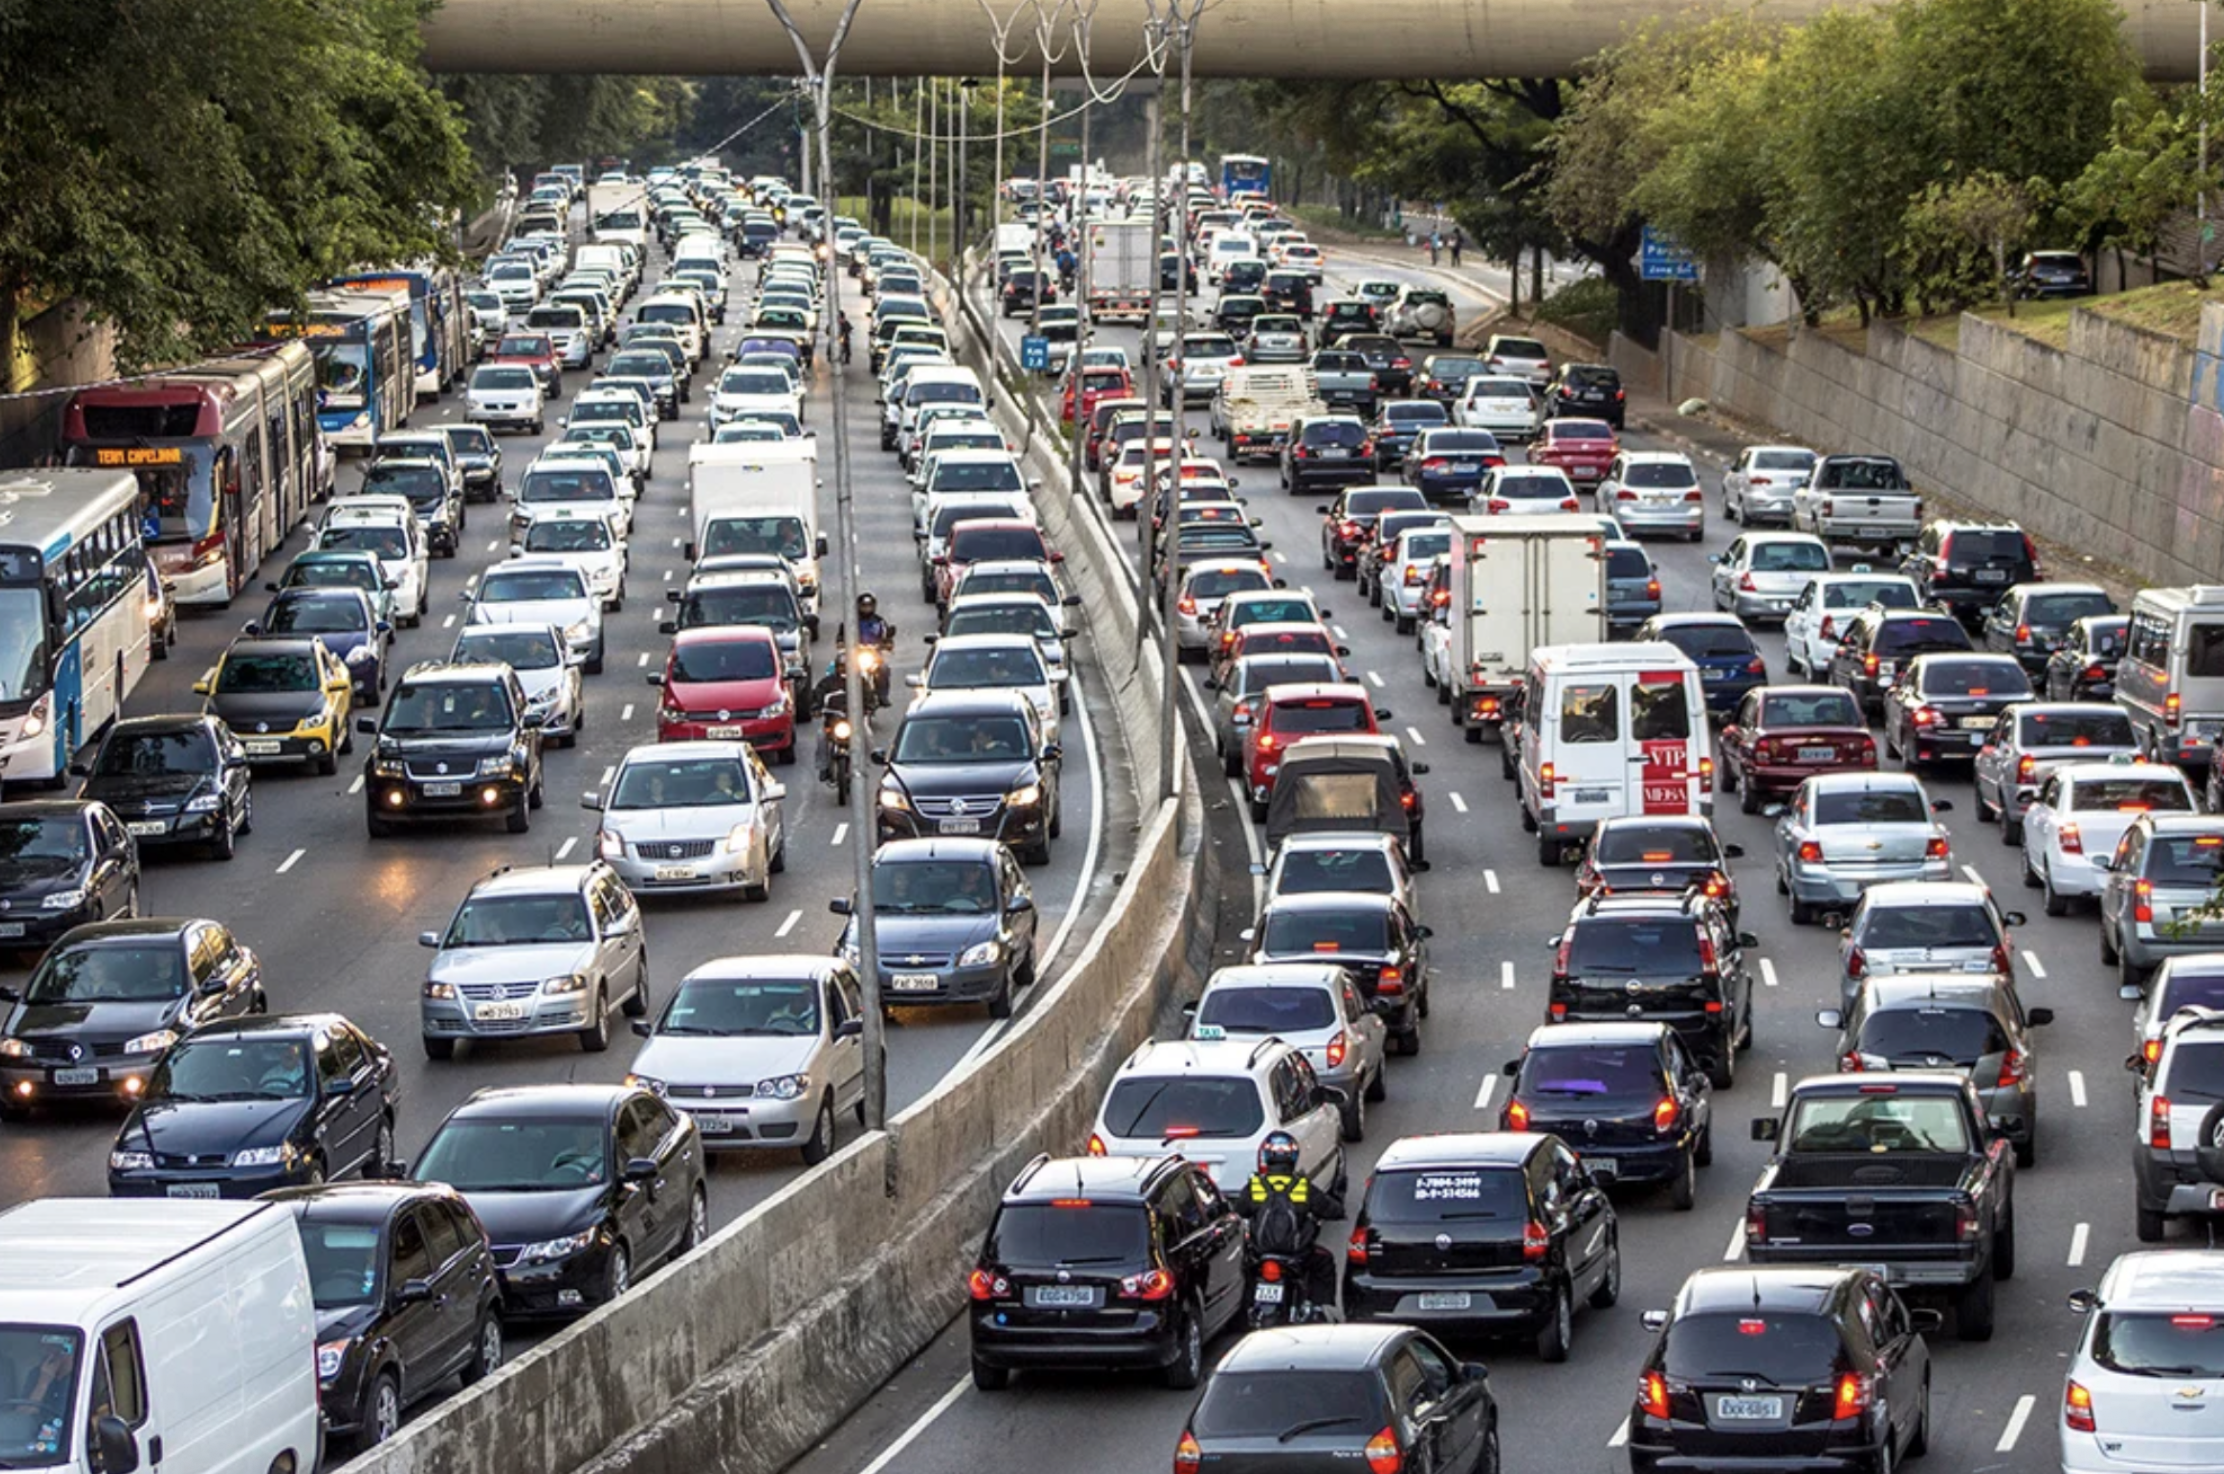
\includegraphics[width=0.4\textwidth]{assets/ch3/1.png}
    \caption{The modeling cycle.}
    \label{fig:ch3_modeling_cycle}
\end{figure}

The \textbf{world} is the environment where the simulation is executed. It contains not only the physical specifications but also the behavioral rules of the objects that compose it. Each decision influences the movement restrictions between agents and the interactions they can have with each other and with the environment itself. We have four types of environments:
\begin{itemize}
    \item \textbf{Discrete space} (cellular space, grid), where space is divided into cells;
    \item \textbf{Continuous space}, where agents can move freely in a continuous environment
    \item \textbf{Geographic space} (GIS), which represents real-world geographical features;
    \item \textbf{Topological space} (network), where agents are nodes connected by edges.
\end{itemize}

\begin{figure}[H]
    \centering
    \includegraphics[width=0.4\textwidth]{assets/ch3/2.png}
    \caption{Types of environments in agent-based modeling.}
    \label{fig:ch3_environment_types}
\end{figure}

A minimum time unit, the \textbf{step}, is assumed. In each step, agents can execute the actions they require, even if they don't have to follow the same order in each iteration of the simulation. A step:
\begin{itemize}
    \item Must capture everything required by our simulation;
    \item Should be as short as possible;
    \item Is the same for every agent.
\end{itemize}

Agents can communicate with each other using \textbf{messages}, which can be direct (one-to-one) or broadcast (one-to-many). Communication can be synchronous (waiting for a response) or asynchronous (not waiting). The choice of communication method depends on the model's requirements and the desired level of interaction among agents. We have to keep in mind the distance, connectivity, information loss and other factors that can affect communication. 
Moreover, how are resources exchanged between agents? How is the behavior of agents modeled?

\section{ODD Protocol}

It is complicated to establish and communicate all the necessary characteristics of the model. An incomplete description eliminates \textbf{replicability}, and a non-reproducible model is not scientific. 
The \textbf{ODD Protocol} (Overview, Design concepts, Details) is a standardized framework for describing agent-based models. It provides a structured approach to document the key components and processes of the model, ensuring clarity and reproducibility. The ODD Protocol consists of three main sections:
\begin{itemize}
    \item \textbf{Overview}: This section provides a high-level summary of the model, including its purpose, key entities, and processes. It outlines the main objectives of the model and the questions it aims to address.
    \item \textbf{Design Concepts}: This section delves into the theoretical underpinnings of the model. It discusses the fundamental concepts and principles that guide the design of the model, such as agent behaviors, interactions, and decision-making processes.
    \item \textbf{Details}: This section provides a comprehensive description of the model's implementation. It includes information on the model's structure, algorithms, parameters, and data sources. It also outlines the steps taken to validate and verify the model.
\end{itemize}

\begin{figure}[H]
    \centering
    \includegraphics[width=0.5\textwidth]{assets/ch3/3.png}
    \caption{The ODD Protocol structure.}
    \label{fig:ch3_odd_protocol}
\end{figure}

\paragraph{Pros of ABM} Hypotheses are expressed at the individual level, allowing for detailed representation of agent behaviors and interactions. This bottom-up approach enables the emergence of complex system dynamics from simple local rules. We can model the evolution of the system and models are experimental objects (simulations).

\paragraph{Cons of ABM} Difficulty to reproduce the complexity of reality (micro/macro levels). High computational cost for large-scale simulations. Validation and verification can be challenging due to the stochastic nature of agent interactions.

ABM should be applied when:
\begin{itemize}
    \item The system is composed of heterogeneous and autonomous entities;
    \item It is difficult to test hypothesis based solely on observations of the real system;
    \item It is possible to identify intermediate variables that link micro-level behaviors to macro-level outcomes;
    \item The relationships among entities are non-linear and dynamic;
    \item Changes at the macro level must be results, not inputs, of the model.
\end{itemize}

